\documentclass[12pt]{article}

% --- Packages ---
\usepackage[utf8]{inputenc}
\usepackage[T1]{fontenc}
\usepackage[french]{babel}
\usepackage{amsmath, amssymb}
\usepackage{geometry}
% \usepackage[draft]{graphicx}
\usepackage{tikz}
\usepackage[most]{tcolorbox}
\usepackage{multicol}
\usepackage{lmodern}
\usepackage{pgfplots}
\pgfplotsset{compat=1.18}
\usepackage{mdframed}
\usepackage{array}
\usepackage[thinlines]{easytable}
\usepackage{tkz-tab}
\usepackage{bm}
\usepackage{xcolor}
\usepackage{sectsty}
\usepackage[utf8]{inputenc}
\usepackage[T1]{fontenc}
\usepackage[inline]{enumitem}
\usepackage[dvipsnames]{xcolor}
\usepackage{multido}
% --- Page ---
\geometry{margin=2cm}

% Footer
\usepackage{fancyhdr}
\pagestyle{fancy}
\cfoot{\thepage}
\rfoot{\textit{G.M.}}
\renewcommand{\headrulewidth}{0pt}
\renewcommand{\footrulewidth}{0pt}

% Pour les normes : 
\newcommand*{\norme}[1]{\left\lVert\overrightarrow{#1}\right\rVert}

\usetikzlibrary{shapes.misc}

\tikzset{cross/.style={cross out, draw=black, minimum size=2*(#1-\pgflinewidth), inner sep=0pt, outer sep=0pt},
%default radius will be 1pt. 
cross/.default={4pt}}

% mettre dans le préambule, après \usepackage{xcolor}
\usepackage{sectsty} % gère facilement la couleur des titres
\setlength{\parindent}{0pt}

\sectionfont{\color{red}\Large\bfseries}     % pour \section*
\subsectionfont{\color{red}\large\bfseries\hspace{1cm}}

\begin{document}

% ============================
%   Probabilités
% ============================

\newpage

\begin{center}
    {\LARGE \textbf{Systèmes d'équations}}\\[4mm]
    {\large - 2\up{nde} -}
\end{center}

\vspace{10pt}
\hrule
\vspace{0pt}

\vspace{20pt}

{\color{RedOrange}\textbf{\underline{Exemple d'introduction :}}}

\vspace{10pt}
Soit deux équations à deux inconnues $x$ et $y$ :
$2x - y = 0$ et $3x - 4y = -5$.

\vspace{5pt}
Elles forment ce qu’on appelle un système de deux équations à \textbf{deux inconnues}.

\vspace{5pt}
\underline{Et on note :}
$$
\left\{
    \begin{array}{ll}
        2x - y = 0 \\
        3x - 4y = -5
    \end{array}
\right.
$$

Un couple de nombres qui vérifie les deux équations est appelé solution du système.
Ici, \textbf{le couple ({\color{blue}1} ; {\color{red}2}) est solution}. 

\vspace{10pt}
\underline{En effet :}
$$
\left\{
    \begin{array}{ll}
        2 \times {\color{blue}1} - {\color{red}2} = 0 \\
        3 \times {\color{blue}1} - 4 \times {\color{red}2} = -5
    \end{array}
\right.
$$

\vspace{10pt}
Dans ce chapitre, on verra deux méthodes permettant de résoudre de tels systèmes.

% ============================
%   Partie 1 : Rappels sur les probabilités
% ============================

\section*{\textcolor{red}{I/ Méthode de substitution}}

\vspace{5pt}

{\color{RedOrange}\textbf{\underline{Méthode :} Résoudre un système par la méthode de la substitution.}}

\vspace{5pt}
On cherche à résoudre le système suivant :
$$
\left\{
    \begin{array}{ll}
        3x + 2y = 0 \\
        x - 4y = 14
    \end{array}
\right.
$$

{\color{red}\underline{\textbf{À RETENIR :}}} Un système est un \textbf{bloc}, on le réécrit à chaque étape 
\underline{\textbf{EN ENTIER}}.

\vspace{5pt}
\textbullet \ On isole une des deux inconnues (la plus simple !) :

\vspace{0.5cm}
{\color{black!45}\dotfill}

\vspace{0.5cm}
{\color{black!45}\dotfill}

\vspace{0.5cm}
{\color{black!45}\dotfill}

\vspace{20pt}

\vspace{5pt}
\textbullet \ On remplace (ou substitue) $x$ par sa valeur dans la 1\up{ère} équation : 

\vspace{0.5cm}
{\color{black!45}\dotfill}

\vspace{0.5cm}
{\color{black!45}\dotfill}

\vspace{0.5cm}
{\color{black!45}\dotfill}

\vspace{20pt}

\textbullet \ On peut alors résoudre la 1\up{ère} équation et trouver $y$ : 

\vspace{0.5cm}
{\color{black!45}\dotfill}

\vspace{0.5cm}
{\color{black!45}\dotfill}

\vspace{0.5cm}
{\color{black!45}\dotfill}

\vspace{0.5cm}
{\color{black!45}\dotfill}

\vspace{0.5cm}
{\color{black!45}\dotfill}

\vspace{20pt}

\textbullet \ Et on susbtitue cette fois-ci y dans la 2\up{ème} équation pour finir la résolution : 

\vspace{0.5cm}
{\color{black!45}\dotfill}

\vspace{0.5cm}
{\color{black!45}\dotfill}

\vspace{0.5cm}
{\color{black!45}\dotfill}

\vspace{20pt}

La solution de ce systèmes est donc {\color{black!45}\dotfill}

\vspace{20pt}
\begin{mdframed}[
    linewidth=1pt,
    roundcorner=5pt,
    linecolor=RoyalBlue,
    innertopmargin=10pt,
    innerbottommargin=10pt
]
{\color{RoyalBlue}
\textbf{\underline{Exercice d'application n°1:} Résoudre un système d'équation avec la méthode de substitution.}}

\vspace{5pt}
Résoudre le système suivant par substitution :
$$
\left\{
    \begin{array}{ll}
        -2x + y -1 = 0 \\
        3x - 4y +2 = 0
    \end{array}
\right.
$$

\vspace{0.5cm}
{\color{black!45}\dotfill}

\vspace{0.5cm}
{\color{black!45}\dotfill}

\vspace{0.5cm}
{\color{black!45}\dotfill}

\vspace{0.5cm}
{\color{black!45}\dotfill}

\vspace{0.5cm}
{\color{black!45}\dotfill}

\vspace{0.5cm}
{\color{black!45}\dotfill}

\vspace{20pt}

\end{mdframed}


\vspace{10pt}
\section*{\textcolor{red}{II/ Méthode des combinaisons linéaires}}

{\color{RedOrange}\textbf{\underline{Méthode :} Résoudre un système d'équation par la méthode des combinaisons
linéaires}}

\vspace{5pt}
On cherche à résoudre le système suivant : 

$$
\left\{
    \begin{array}{ll}
        3x - 2y =11\\
        6x + 3y = 15
    \end{array}
\right.
$$

\vspace{5pt}
Est-il possible d'appliquer la méthode par susbtitution simplement ici ? Pourquoi ?

\vspace{0.5cm}
{\color{black!45}\dotfill}

\vspace{0.5cm}
{\color{black!45}\dotfill}

\vspace{20pt}

Nommons les deux lignes du système : $\bm{L_1}$ et $\bm{L_2}$ :

$$
\left\{
    \begin{array}{ll}
        3x - 2y =11 & L_1\\
        6x + 3y = 15 & L_2
    \end{array}
\right.
$$

Remarquons maintenant un lien entre ces deux lignes au niveau des $x$... 

\vspace{0.5cm}
{\color{black!45}\dotfill}

\vspace{0.5cm}
{\color{black!45}\dotfill}

\vspace{20pt}

\textbullet \ Multiplions $L_1$ pour se retrouver avec le même coefficient pour les $x$ : 

\vspace{0.5cm}
{\color{black!45}\dotfill}

\vspace{0.5cm}
{\color{black!45}\dotfill}

\vspace{20pt}

\textbullet \ On peut maintenant soustraire les deux lignes dans l'ordre que l'on veut :

\vspace{0.5cm}
{\color{black!45}\dotfill}

\vspace{0.5cm}
{\color{black!45}\dotfill}

\vspace{0.5cm}
{\color{black!45}\dotfill}

\vspace{20pt}

\textbullet \ Enfin, on remplace $y$ dans l'équation que l'on veut : 

\vspace{0.5cm}
{\color{black!45}\dotfill}

\vspace{0.5cm}
{\color{black!45}\dotfill}


\vspace{20pt}
La solution du système est le couple \_\_\_\_\_\_\_\_\_\_\_\_. On note : 

\vspace{20pt}
On cherche maintenant à résoudre le système suivant : 

$$
\left\{
    \begin{array}{ll}
        3x - 2y = 7 \\
        5x + 3y = -1
    \end{array}
\right.
$$

\vspace{0.5cm}
{\color{black!45}\dotfill}

\vspace{0.5cm}
{\color{black!45}\dotfill}

\vspace{20pt}

On multiplie $L_1$ par \_\_\_\_\_\_\_ et $L_2$ par \_\_\_\_\_\_\_

\vspace{0.5cm}
{\color{black!45}\dotfill}

\vspace{0.5cm}
{\color{black!45}\dotfill}

\vspace{0.5cm}
{\color{black!45}\dotfill}


\vspace{20pt}
On peut alors {\color{black!45}\dotfill}

\vspace{0.5cm}
{\color{black!45}\dotfill}

\vspace{0.5cm}
{\color{black!45}\dotfill}

\vspace{0.5cm}
{\color{black!45}\dotfill}

\vspace{20pt}
Et enfin {\color{black!45}\dotfill}

\vspace{0.5cm}
{\color{black!45}\dotfill}

\vspace{0.5cm}
{\color{black!45}\dotfill}

\vspace{20pt}

La solution du système est le couple \_\_\_\_\_\_\_\_\_\_\_\_. On note : 

\vspace{20pt}
\vspace{10pt}
\section*{\textcolor{red}{III/ Cas particuliers et lien graphique}}

\subsection*{1) Système admettant une unique solution}
\vspace{5pt}

Résolvons le système suivant : 
$$
\left\{
    \begin{array}{ll}
        -2x + y = 0 \\
        4x - y = 4
    \end{array}
\right.
$$

\vspace{0.5cm}
{\color{black!45}\dotfill}

\vspace{0.5cm}
{\color{black!45}\dotfill}

\vspace{0.5cm}
{\color{black!45}\dotfill}

\vspace{0.5cm}
{\color{black!45}\dotfill}

\vspace{0.5cm}
{\color{black!45}\dotfill}

\vspace{0.5cm}
{\color{black!45}\dotfill}

\vspace{20pt}

On trouve donc une solution unique : \_\_\_\_\_\_\_\_\_\_\_\_

\vspace{20pt}
\underline{Reprenons ce même système et isolons maintenant $y$ pour les deux lignes :} 

\begin{minipage}[t]{.5\textwidth}%
    \vspace{30pt}
    $$
    \left\{
        \begin{array}{ll}
            -2x + y = 0 \\
            4x - y = 4
        \end{array}
    \right.
    $$

    \vspace{0.5cm}
    {\color{black!45}\dotfill}

    \vspace{0.5cm}
    {\color{black!45}\dotfill}

    \vspace{0.5cm}
    {\color{black!45}\dotfill}
    

    \vspace{20pt}
    Nous trouvons deux équations de droites. Que l'on peut représenter comme ci-contre : 
\end{minipage}%
\hfill
\begin{minipage}[t]{.5\textwidth}%
    \vspace{-10pt}
    \begin{center}
        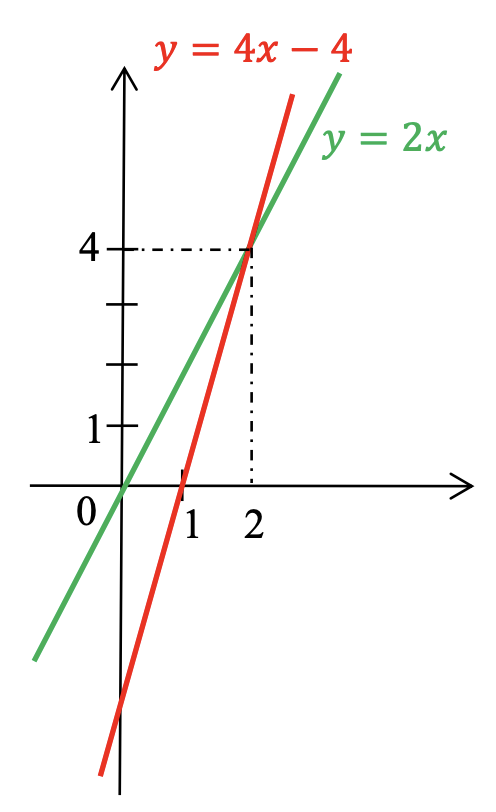
\includegraphics[width=0.6\textwidth]{fig1.png}
    \end{center}
\end{minipage}%

{\color{red}\underline{\textbf{À RETENIR :}}} la solution du système est donc le couple 
$(x ; y)$ coordonnées du \textbf{point d'intersection} des deux droites.

\vspace{10pt}
\subsection*{2) Système n'admettant pas de solutions}
\vspace{5pt}

Résolvons le système suivant : 
$$
\left\{
    \begin{array}{ll}
        y = 3x + 1 \\
        -2y = -6x + 6
    \end{array}
\right.
$$

\vspace{0.5cm}
{\color{black!45}\dotfill}

\vspace{0.5cm}
{\color{black!45}\dotfill}

\vspace{0.5cm}
{\color{black!45}\dotfill}

\vspace{20pt}

On aboutit à une \textbf{absurdité} :
{\color{black!45}\dotfill}


\vspace{20pt}
\underline{Reprenons ce même système et isolons maintenant $y$ pour les deux lignes :} 

\begin{minipage}[t]{.5\textwidth}%
    \vspace{0pt}
    $$
    \left\{
        \begin{array}{ll}
            y = 3x + 1 \\
            -2y = -6x + 6
        \end{array}
    \right.
    $$

    \vspace{0.5cm}
    {\color{black!45}\dotfill}

    \vspace{0.5cm}
    {\color{black!45}\dotfill}

    \vspace{0.5cm}
    {\color{black!45}\dotfill}
    
    \vspace{0.5cm}
    {\color{black!45}\dotfill}
    
    \vspace{0.5cm}
    {\color{black!45}\dotfill}
    

    \vspace{20pt}
\end{minipage}%
\hfill
\begin{minipage}[t]{.5\textwidth}%
    \vspace{0pt}
    \begin{center}
        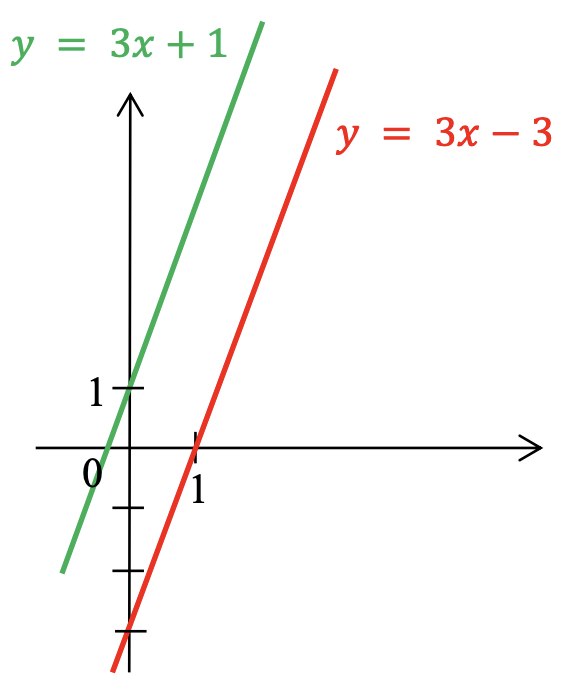
\includegraphics[width=0.6\textwidth]{fig2.png}
    \end{center}
\end{minipage}%

{\color{red}\underline{\textbf{À RETENIR :}}} les droites n'ont pas de points d'intersection 
donc le système n'a pas de solutions.

\vspace{20pt}
On note : \_\_\_\_\_\_\_\_\_\_\_\_

\subsection*{3) Système admettant une infinité de solutions}
\vspace{5pt}

Résolvons le système suivant : 
$$
\left\{
    \begin{array}{ll}
        -6x -3y = -6 \\
        2x + y = 2
    \end{array}
\right.
$$

\vspace{0.5cm}
{\color{black!45}\dotfill}

\vspace{0.5cm}
{\color{black!45}\dotfill}

\vspace{0.5cm}
{\color{black!45}\dotfill}

\vspace{20pt}

On aboutit à une \textbf{évidence} :
{\color{black!45}\dotfill}


\vspace{20pt}
\underline{Reprenons ce même système et isolons maintenant $y$ pour les deux lignes :} 

\begin{minipage}[t]{.5\textwidth}%
    \vspace{0pt}
    $$
    \left\{
        \begin{array}{ll}
            -6x -3y = -6 \\
            2x + y = 2
        \end{array}
    \right.
    $$

    \vspace{0.5cm}
    {\color{black!45}\dotfill}

    \vspace{0.5cm}
    {\color{black!45}\dotfill}

    \vspace{0.5cm}
    {\color{black!45}\dotfill}
    
    \vspace{0.5cm}
    {\color{black!45}\dotfill}
    
    \vspace{0.5cm}
    {\color{black!45}\dotfill}
    

    \vspace{20pt}
\end{minipage}%
\hfill
\begin{minipage}[t]{.5\textwidth}%
    \vspace{0pt}
    \begin{center}
        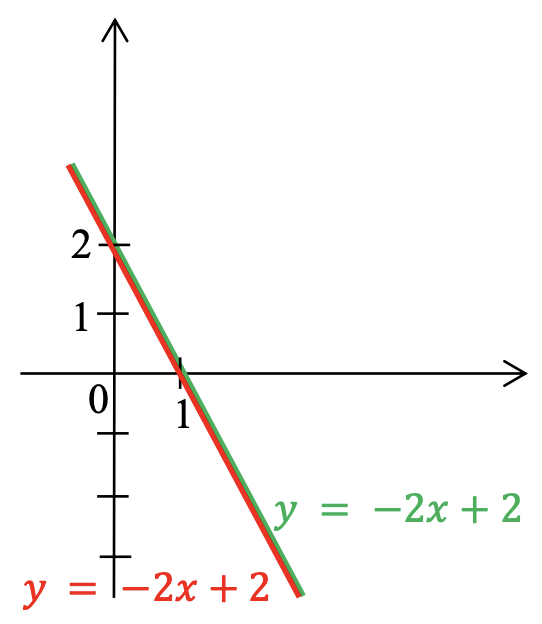
\includegraphics[width=0.6\textwidth]{fig3.png}
    \end{center}
\end{minipage}%

{\color{red}\underline{\textbf{À RETENIR :}}} les droites ont la même équation, elles sont donc

\vspace{20pt}\_\_\_\_\_\_\_\_\_\_\_\_. 

\vspace{20pt}
Elles possède une infinité de \_\_\_\_\_\_\_\_\_\_\_\_\_\_\_\_\_\_\_\_\_\_\_\_

\vspace{20pt}
Le système possède dont une infinité de solutions : \_\_\_\_\_\_\_\_\_\_\_\_\_\_\_\_\_\_\_\_\_\_\_\_





\end{document}
